\chapter{Predchádzajúce riešenia}

\section{Verifikačný softvér}

Verifikácia predpovedných modelov počasia je úloha dokonale stvorená pre automatizáciu. 
Z tohto dôvodu meteorológovia začali využívať dostupný štatistický softvér 
a neskôr boli taktiež vyvíjané špecializované nástroje určené pre verifikáciu.
Môžeme teda rozdeliť verifikačný softvér do dvoch základných kategórií a to \textit{štatistický} a \textit{špecializovaný}, ktorý je zväčša podporovaný rôznymi národnými a medzinárodnými organizáciami.

\subsection{Štatistický softvér}
%TODO
Spoločnou črtou: \\
	- obmedzená funkcionalita \\
	- obmedzená vizualizácia \\
	- slabé / žiadne GUI \\
	- vyžaduje znalosť špecifického programovacieho jazyka \\
	- ...


\subsubsection{Tabuľkový softvér}
Napriek tomu, že je tabuľkový softvér na výpočet štatistík zamietnutý komunitou vedcov a štatistikov ako nevhodný a neprofesionálny, tak je využívaný, a to pomerne často, aj vo vedeckých kruhoch. 
Výhodou je, že novému užívateľovi umožňuje okamžite vidieť všetky kroky v základných procedúrach verifikácie a teda je výborný pre výučbové účely. \cite{VerifSoft} 
Najznámejší kus softvéru z pomedzi komerčných produktov je \textit{Microsoft Excel}[ref] a z voľne dostupných je jeho opensoruce náprotivok \textit{Open Office Calculate}[ref]. Oba programy zahrňujú základné štatistické funkcie ako napríklad stredná kvadratická chyba (\textit{MSE}) pre spojité predpovede (pozri odsek \ref{subsec:mse}) a taktiež umožňujú generovanie jednoduchých grafov na základe tabuľkových dát. Tabuľkový softvér neposkytuje priamo funkcionalitu na výpočet ďalších sofistikovanejších verifikačných štatistík, avšak umožňuje ich implementáciu pomocou makro programovania v špecifickom jazyku. Pre Microsoft Excel je to \textit{Microsoft Visual Basic}[ref] a pre Open Office Calculate zasa \textit{OpenOffice.org Basic}[ref]. Oba jazyky patria do rodiny \textit{Basic} jazykov, takže majú mnoho podobných prvkov.  


\subsubsection{MATLAB}
\textit{MATLAB} je interaktívne prostredie s vlastným programovacím jazykom, ktorý je využívaný miliónmi inžinierov a vedcov po celom svete [ref] a tým nevynímajúc meteorológov a ďalších odborníkov pracujúcich v atmosférickom výskume. 
Zvyčajne sa MATLAB využíva na výskum a protoypovanie nových metód a procedúr \cite{VerifSoft}, pretože umožňuje rýchlu a jednoduchú implementáciu, keďže jeho súčasťou je mnoho matematických knižníc a je prispôsobený na prácu s maticami dát.
Výhodou MATLABU je, že umožňuje tvorbu GUI a taktiež poskytuje kreslenie rôznorodých grafov a diagramov.
Mali by sme však podotknúť, že podobne ako väčšina štatistického softvéru, aj \textit{MATLAB} je komerčný produkt. Jeho cena za jednu licenciu je \$2,650 (k roku 2015), čo je pomerne vysoká suma, ak vezmeme do úvahy za akým účelom chceme tento softvér využívať a ako dobre je naň prispôsobený.

\subsubsection{Minitab} % Toto tu netreba!


\subsubsection{R}

\subsubsection[SAS]{Statistical Analysis Software (SAS)}

\subsubsection[IDL]{Interactive Data Language (IDL)}

\subsection{Špecializovaný softvér}

\subsubsection[NCL]{NCAR Command Language (NCL)}

\subsubsection[MET]{Model Evaluation Tools (MET)}

\subsubsection[EVS]{Ensemble Verification System (EVS)}


%TODO tabuľka softvéru

\section{Vizualizácia verifikácie}

\subsection{Scatterplot}

\subsection{Krabicový graf}
Krabicový graf je v anglickej literatúre zvyčajne nazývaný \textit{box plot} alebo na niektorých miestach označovaný tiež ako \textit{box and whisker\footnote{Slovo \textit{whisker} znamená po slovensky fúz, čo nám naznačuje, že čiary, ktoré spájajú horný a dolný kvartál s hraničnými hodnotami pripomínajú fúzy.} plot}. Odkedy bol prvýkrát publikovaný v roku 1977 [Tukey], uplynulo už takmer 40 rokov a dnes ho považujeme už za štandardnú techniku ako vizualizovať distribúciu hodnôt kompaktným spôsobom. Na svoju reprezentáciu využíva súbor 5 čísel (tzv. \textit{5-number summary})[Potter], ktoré charakterizujú distribúciu dát robustným spôsobom. Tým, že zredukujeme zvyčajne veľkú dátovú množinu na týchto pár hodnôt ušetríme nielen vzácny vizuálny priestor [Wickham], ale taktiež námahu analytika, ktorý sa snaží preskúmať iba niektoré vybrané charakteristiky. 

\subsubsection{Konštrukcia krabicového diagramu}

Na zostavenie krabicového diagramu potrebujeme týchto 5 hodnôt: medián, horný kvartál a dolný kvartál, maximum, minimum. (pozri obrázok \ref{fig:boxplot}) Prvé tri hodnoty sú takzvané kvartály, ktoré rozdeľujú súbor dát na 4 rovnako veľké časti a ďalšie dve sú extrémne hodnoty, ktoré ohraničujú celý dátový súbor. 

%TODO nakreslit dalsie variacie boxplotu do toho isteho diagramu alebo to dat dalej?

\begin{figure}
	\centering
	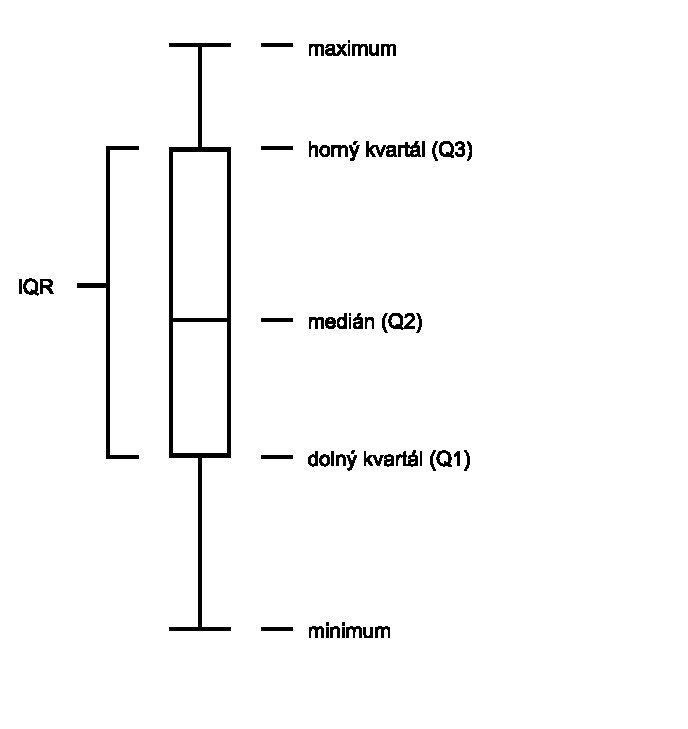
\includegraphics[width = 2.5in]{svg2}
	\caption{Krabicový diagram}
	\label{fig:boxplot}
\end{figure}





\subsection{Time series plot}